\chapter{Experimentos Realizados}
\thispagestyle{plain}
\label{cap:experimentos}
\graphicspath{{./Cap4_Experimentos_Realizados/Figures/}}

A realização dos experimentos baseou-se na utilização da ferramenta de parametrização e obtenção de métricas, aplicado nas imagens tratadas de cada cena, conforme variaçoes definidas no Capítulo anterior. Os dados obtidos foram organizados de forma a facilitar a análise e comparação entre as variaçoes em cada cena e também entre os diferentes dispositivos sendo testados.

Para cada variação de resolução, que depende de uma nova seleção de parâmetros, será exibido a matriz de resultados final juntamente com as faces detectadas, após já feita a análise para se chegar a um melhor resultado, indicando quais foram os parâmetros definidos.

\section{Cena 1}

\subsection{Otimização de parâmetros}

Primeiramente, foi realizada a otimização dos parâmetros para cada variação de resolução, a partir das imagens com todas as faces disponíveis de cada resolução. No caso desta cena, que exige relativamente muito mais processamento, utilizou-se o Raspberry Pi 4B para a definição dos parâmetros, repetindo-os nos testes com o Raspberry Pi Zero W para base de comparação.

A definição dos parâmetros 'ótimos' não é objetiva. Para esta cena, buscou-se um melhor resultado em que houvesse a maior quantidade de faces detectadas com o mínimo ou nenhuma presença de falsos positivos e no menor tempo. Durante a análise, teve-se a razoabilidade de considerar na comparação entre os diferentes resultados da matriz que, um grande aumento no tempo de detecção não justifica um pequeno ganho relativo na quantidade de faces detectadas.

As próximas três subsubseções \ref{sssec:resolution1-1}, \ref{sssec:resolution1-2} e \ref{sssec:resolution1-3} mostram através de imagens, para cada resolução testada, a última iteração da matriz de resultados com os dados entrada, a célula destacada com os parâmetros escolhidos e a imagem com a faces detectadas.

Os parâmetros definidos de cada resolução foram usados para obter as métricas de cada variação de quantidade de faces detectáveis, e em ambos os dispositivos testados. Não será apresentado nesse documento cada resultado das métricas obtidos em tela. Todos os dados foram tabelados e utilizados para as comparações feitas nas subseções seguintes.


\subsubsection{Resolução 1440p} \label{sssec:resolution1-1}

\begin{figure}[H]
    \centering
    \caption[Otimização Cena 1 - resolução 1440p.]{Otimização Cena1 resolução 1440p.}
    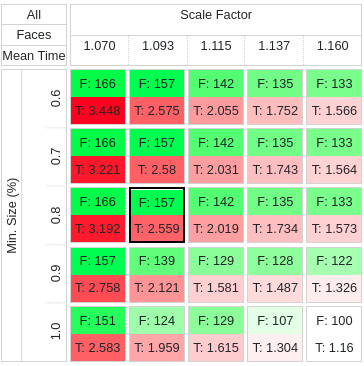
\includegraphics[width=0.85\textwidth]{Cap4_Experimentos_Realizados/Figures/cena1_param_1440p_matriz.jpg}
    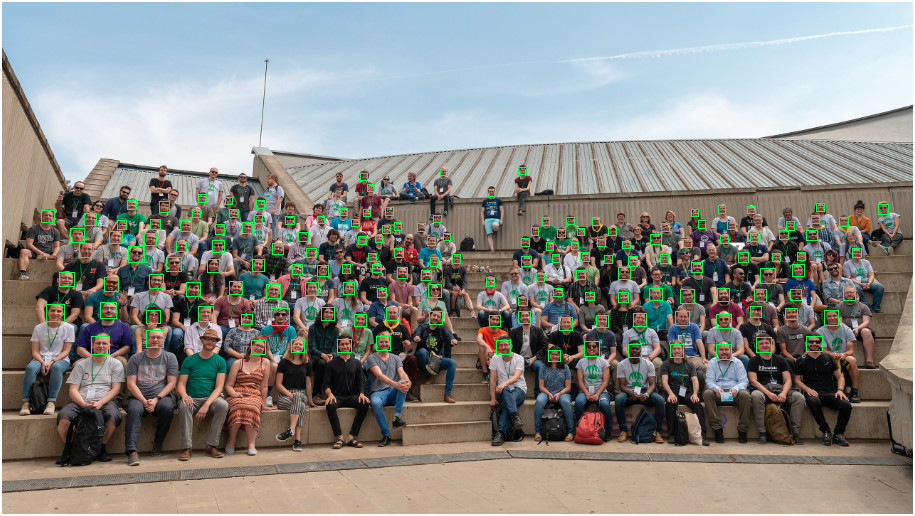
\includegraphics[width=0.85\textwidth]{Cap4_Experimentos_Realizados/Figures/cena1_param_1440p_faces.jpg}
    \caption*{Fonte: autor.}
    \label{fig:otimizacaoCena1_1440p}
\end{figure}

\subsubsection{Resolução 1080p} \label{sssec:resolution1-2}

\begin{figure}[H]
    \centering
    \caption[Otimização Cena 1 - resolução 1080p.]{Otimização Cena1 resolução 1080p.}
    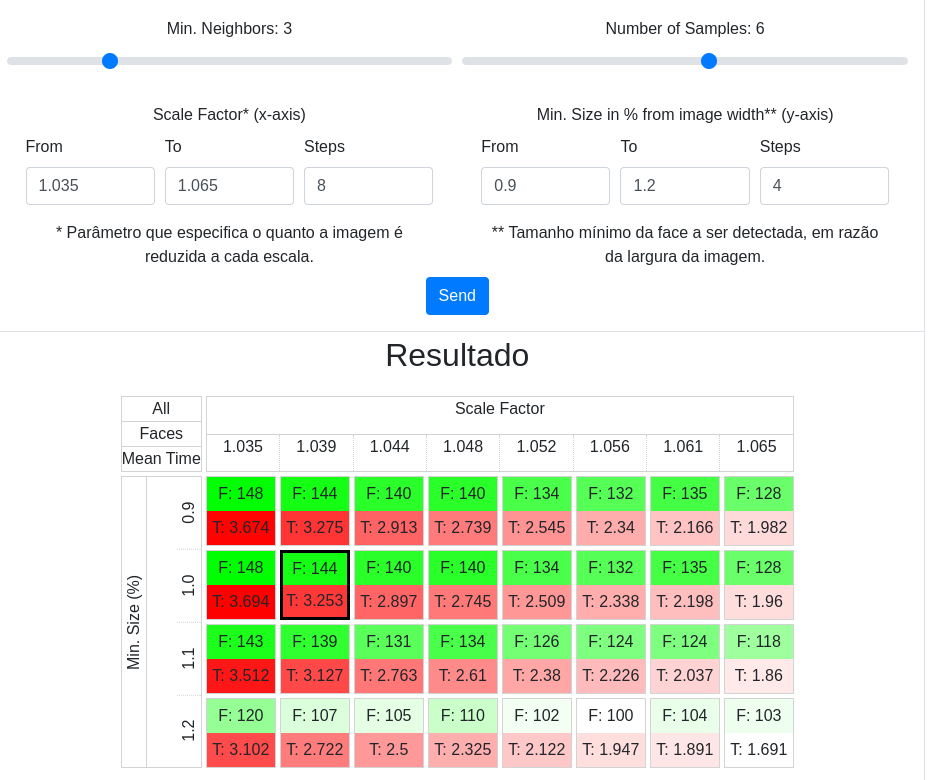
\includegraphics[width=0.85\textwidth]{Cap4_Experimentos_Realizados/Figures/cena1_param_1080p_matriz.jpg}
    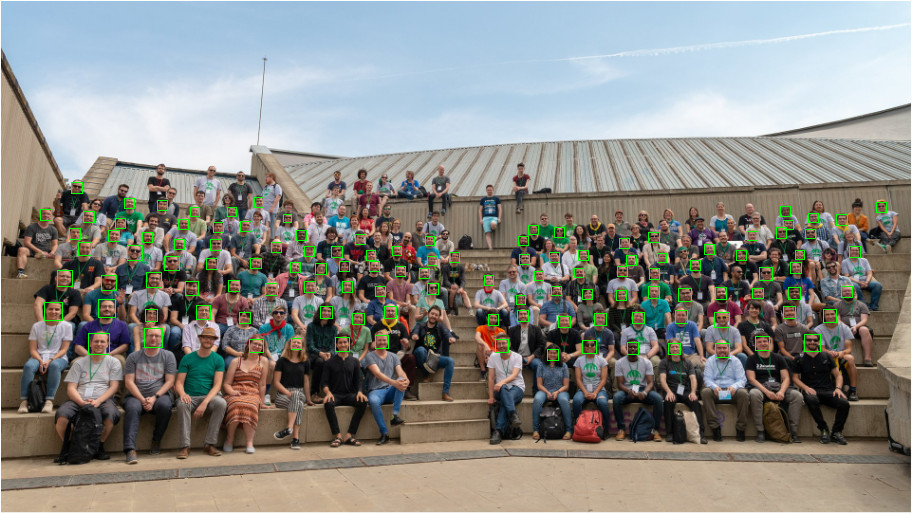
\includegraphics[width=0.85\textwidth]{Cap4_Experimentos_Realizados/Figures/cena1_param_1080p_faces.jpg}
    \caption*{Fonte: autor.}
    \label{fig:otimizacaoCena1_1080p}
\end{figure}

\subsubsection{Resolução 720p} \label{sssec:resolution1-3}

\begin{figure}[H]
    \centering
    \caption[Otimização Cena 1 - resolução 720p.]{Otimização Cena 1 - resolução 720p.}
    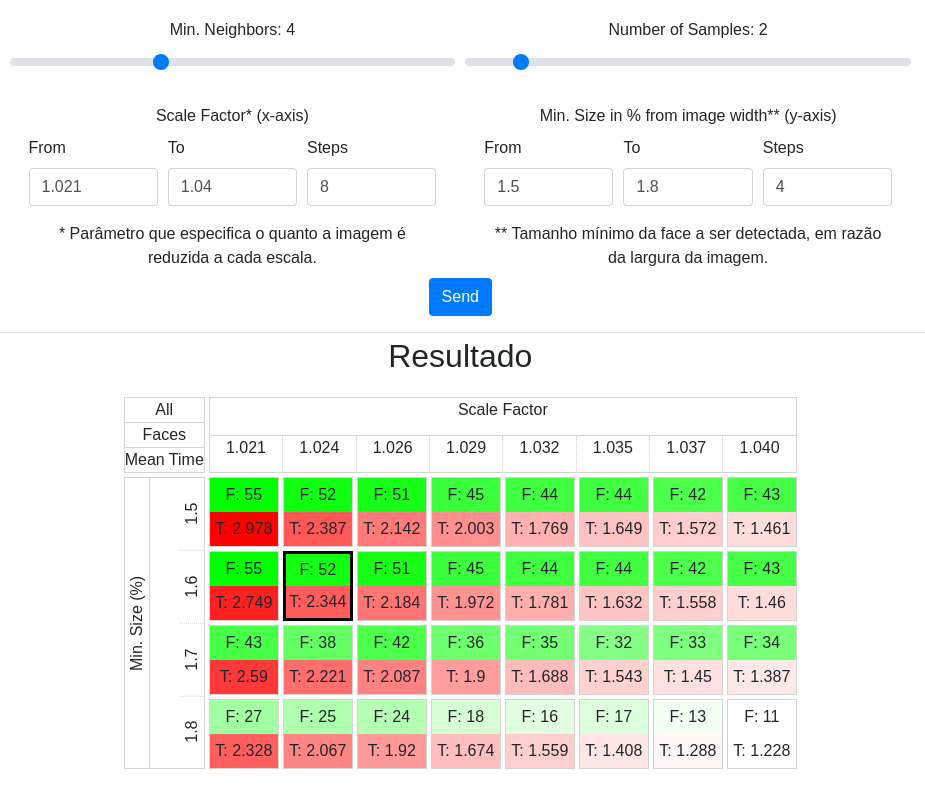
\includegraphics[width=0.85\textwidth]{Cap4_Experimentos_Realizados/Figures/cena1_param_720p_matriz.jpg}
    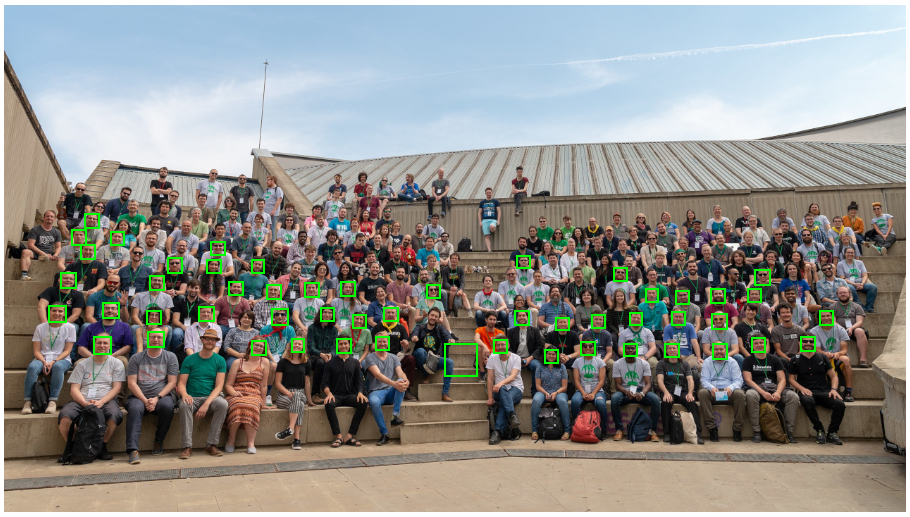
\includegraphics[width=0.85\textwidth]{Cap4_Experimentos_Realizados/Figures/cena1_param_720p_faces.jpg}
    \caption*{Fonte: autor.}
    \label{fig:otimizacaoCena1_720p}
\end{figure}

\section{Cena 2}

\subsection{Captura de imagens para teste}

Conforme definido no capítulo anterior, as imagens para teste foram capturadas a partir de um módulo de câmera conectado no Raspbery Pi 4B.

A cena foi montada conforme pode ser visualizado na figura \ref{fig:cena2_posicao1_visao_externa}. O Raspberry Pi 4B, montado em sua case e com o módulo da câmera conectado foi fixado no batente lateral esquerdo da porta da entrada, de forma que a câmera ficasse posicionada a 1,7m do piso e levemente inclinada para baixo e para a dentro, na direção da passagem. A pessoa que aparece na imagem é o próprio autor.

Utilizando-se o script de captura de frames, foram feitos alguns testes e definiu-se essa como a posição mais próxima para se obter a primeira imagem a ser utilizada nos testes de desempenho, pois consegue pegar uma boa imagem do rosto e ainda com um pouco de folga vertical, considerando-se pessoas mais altas ou baixas.

\begin{figure}[H]
    \centering
    \caption[Posicionamento para captura da face na primeira posição.]{Posicionamento para captura da face na primeira posição.}
    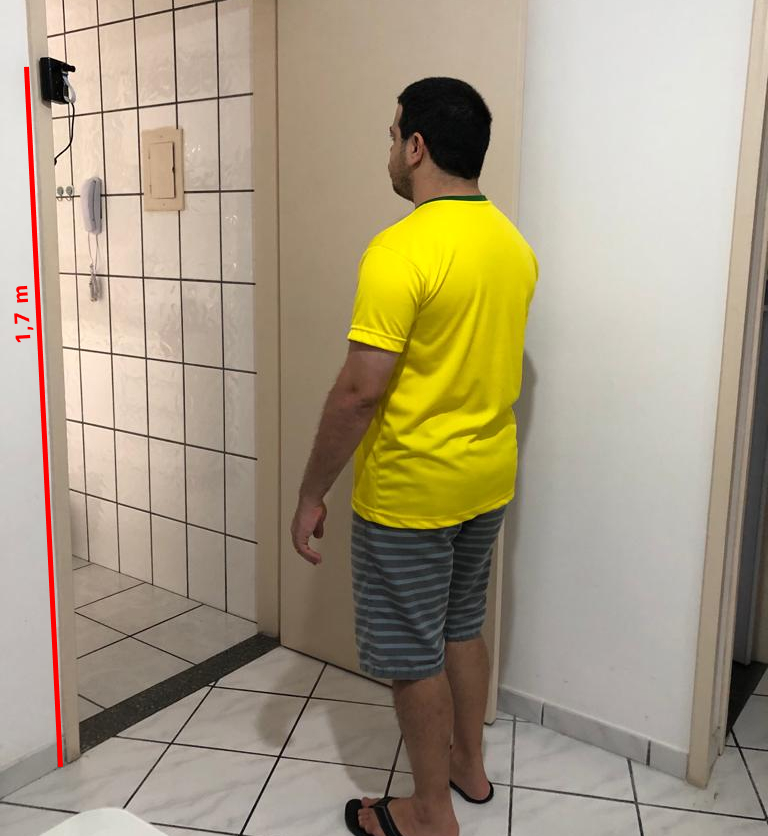
\includegraphics[width=0.65\textwidth]{Cap4_Experimentos_Realizados/Figures/cena2_posicao1_visao_externa.jpg}
    \caption*{Fonte: autor.}
    \label{fig:cena2_posicao1_visao_externa}
\end{figure}

Na figura \ref{fig:cena2_posicao1_imagem_capturada} têm-se a imagem capturada pela câmera na posição 1, na maior resolução definida para esta cena, 800x600.

\begin{figure}[H]
    \centering
    \caption[Captura da imagem na primeira posição.]{Captura da imagem na primeira posição.}
    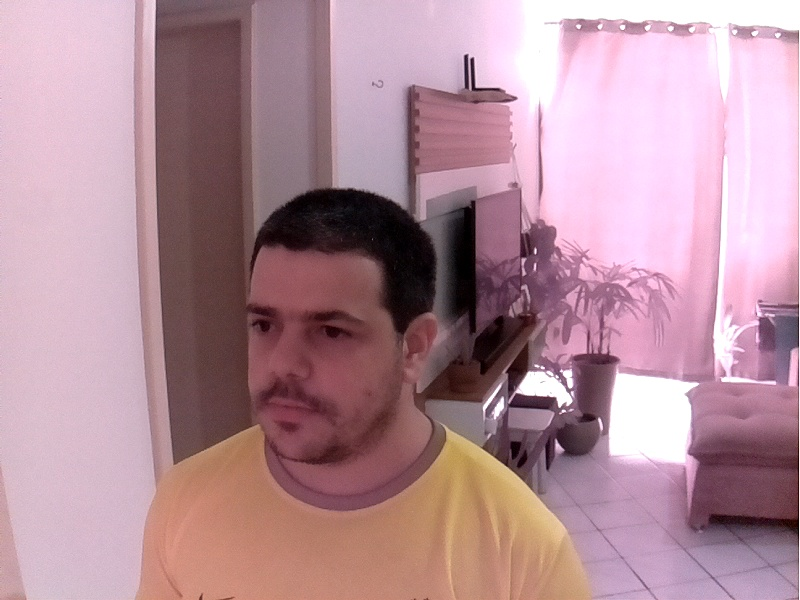
\includegraphics[width=0.65\textwidth]{Cap4_Experimentos_Realizados/Figures/cena2_posicao1_imagem_capturada.jpg}
    \caption*{Fonte: autor.}
    \label{fig:cena2_posicao1_imagem_capturada}
\end{figure}

A partir dessa primeira posição, mediu-se 1,7m distanciando-se da entrada. Essa é a posição mais distante, a partir da qual deseja-se que a face seja detectável. A figura \ref{fig:cena2_posicao2_visao_externa} demonstra esse posicionamento e na figura \ref{fig:cena2_posicao2_imagem_capturada} tem-se a imagem capturada pela câmera que também será utilizada nos testes.
\begin{figure}[H]
    \centering
    \caption[Posicionamento para captura da face na segunda posição.]{Posicionamento para captura da face na segunda posição.}
    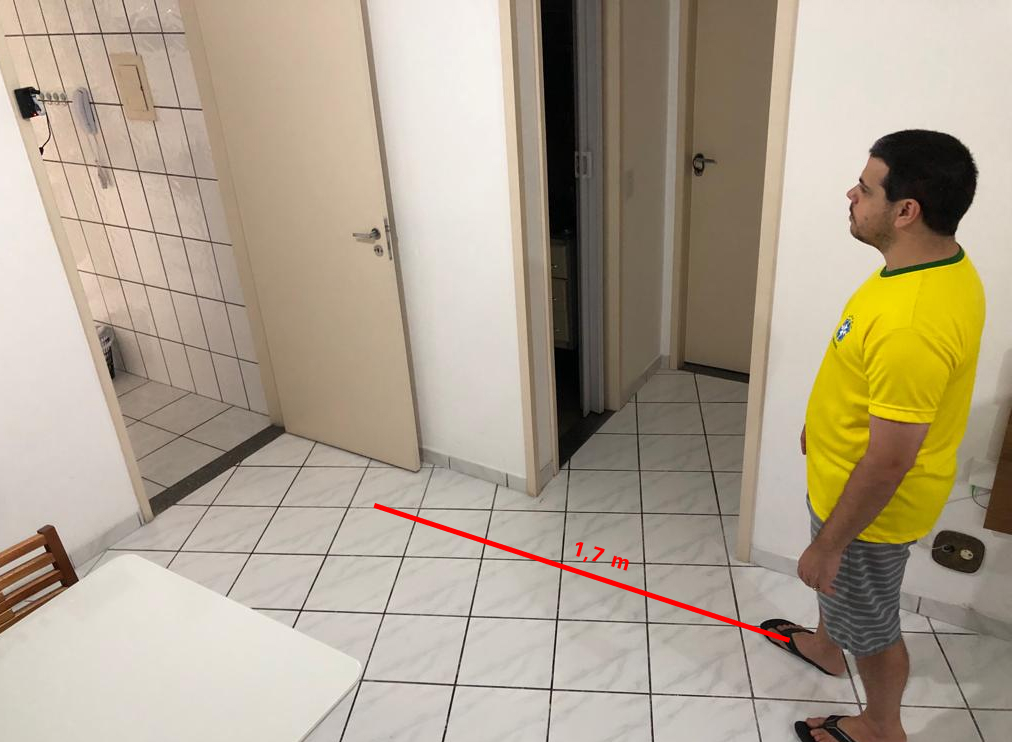
\includegraphics[width=0.65\textwidth]{Cap4_Experimentos_Realizados/Figures/cena2_posicao2_visao_externa.jpg}
    \caption*{Fonte: autor.}
    \label{fig:cena2_posicao2_visao_externa}
\end{figure}

\begin{figure}[H]
    \centering
    \caption[Captura da imagem na segunda posição.]{Captura da imagem na segunda posição.}
    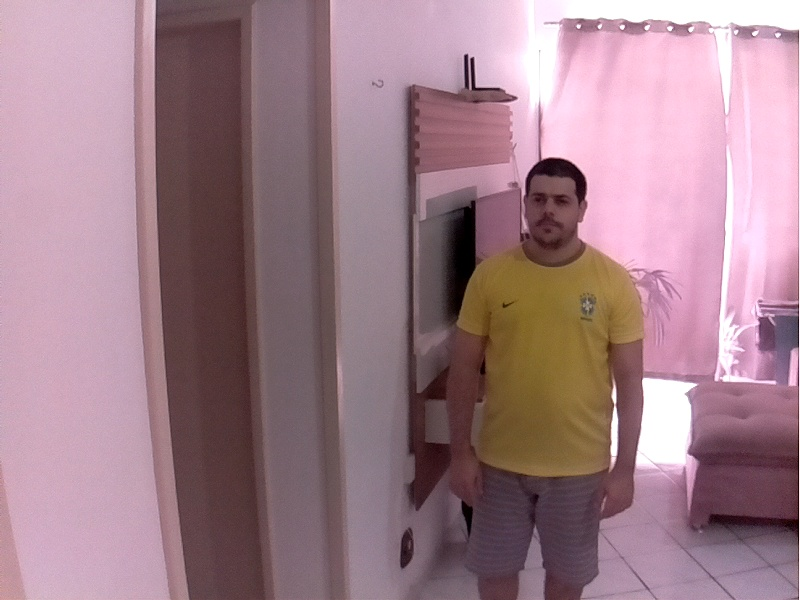
\includegraphics[width=0.65\textwidth]{Cap4_Experimentos_Realizados/Figures/cena2_posicao2_imagem_capturada.jpg}
    \caption*{Fonte: autor.}
    \label{fig:cena2_posicao2_imagem_capturada}
\end{figure}


\subsection{Otimização de parâmetros}

Foi realizada a otimização dos parâmetros para cada variação de resolução, utilizando-se as imagens capturadas nas duas posições. Utilizou-se o Raspberry Pi 4B para a definição dos parâmetros, repetindo-os nos testes com o Raspberry Pi Zero W para base de comparação.

As imagens em ambas as posições foram analisadas em conjunto mas com o objetivo de se chegar a apenas um conjunto de parâmetros 'ótimos' para obtenção das métricas. Foram considerados 'ótimos' a mesma combinação de parâmetros que atendia as duas imagens, buscando-se os limiares com o menor tempo em que as faces são detectadas e sem falsos positivos. Para facilitar a visualização desses limiares, foram definidos passos maiores de ScaleFactor e Min. Size para se obter quantidades maiores de amostras.

Pode-se pensar, a princípio, que bastava analisar a imagem na posição 2, que é a mais distante, pois essa já seria o pior caso, já que a face teria menor resolução que a da posição 1. Porém, percebe-se claramente comparando as figuras \ref{fig:cena2_posicao1_imagem_capturada} e \ref{fig:cena2_posicao2_imagem_capturada} que quando a face está mais próxima da câmera e estando a pessoa olhando naturalmente em direção à entrada, o angulo não é muito bom, podendo criar alguma dificuldade adicional na detecção da face. Por isso a importância da análise conjunta.

Para se considerar um pior caso, foram utilizados os dados das métricas que apresentaram maiores tempos de resposta e tamanho de imagem, isso para cada resolução.

As próximas três subsubseções \ref{sssec:resolution2-1}, \ref{sssec:resolution2-2} e \ref{sssec:resolution2-3} mostram para cada resolução testada, a última iteração da matriz de resultados para a detecção em ambas as posições, com os dados entrada, a célula destacada com os parâmetros escolhidos e as imagems com a faces detectadas.

Após os parâmetros definidos no Raspberry Pi 4, os mesmo foram utilizados para obter a métricas no Raspberry Pi Zero W, sendo todos tabelados para comparação.

\subsubsection{Resolução 600p} \label{sssec:resolution2-1}

Devido ao tamanho maior das matrizes de resultados e a necessidade de visualização lado à lado, a parte da interface com os controles de parametrização não foram exibidos. Os prâmetros utilizados foram: "Min. Neighbors: 3", "Number of Samples: 6". Início e fim de escala dos demais parâmetros podem ser vistos nas matrizes.

<pending> nas matrizes foram demarcadas linhas azui e vermelhas ...etc

\begin{figure}[H]
    \centering
    \caption[Otimização Cena 2 - resolução 600p - matrizes. À esquerda posição 1 e à direita, posição 2]{Otimização Cena 2 - resolução 600p - matrizes. À esquerda, posição 1, e à direita, posição 2.}
    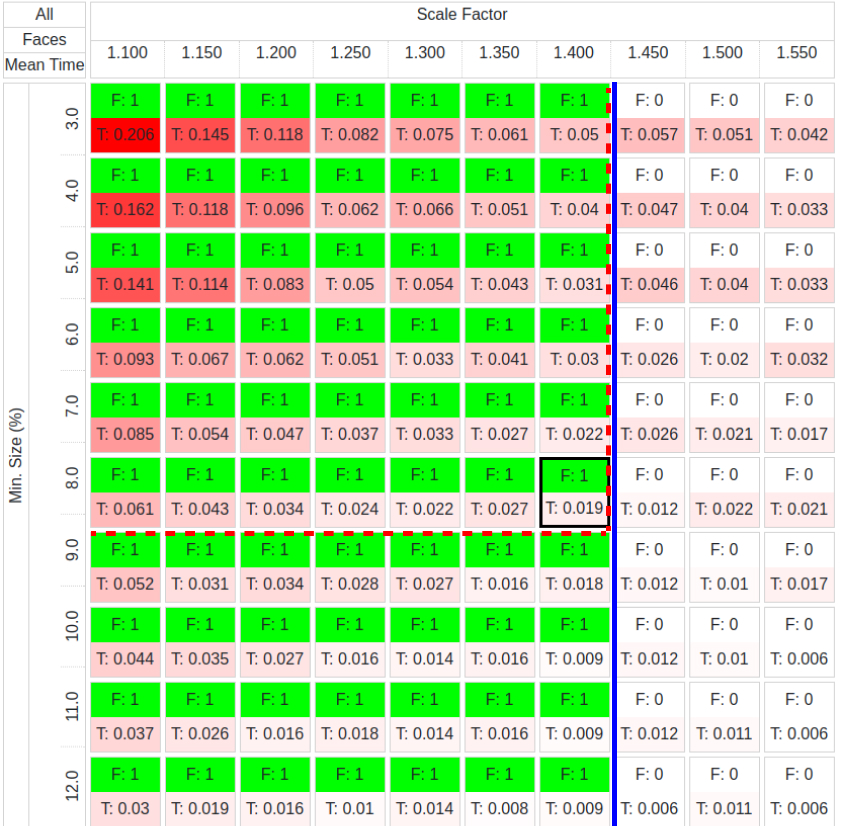
\includegraphics[width=0.49\textwidth]{Cap4_Experimentos_Realizados/Figures/cena2_800x600_pos1_matriz.jpg}
    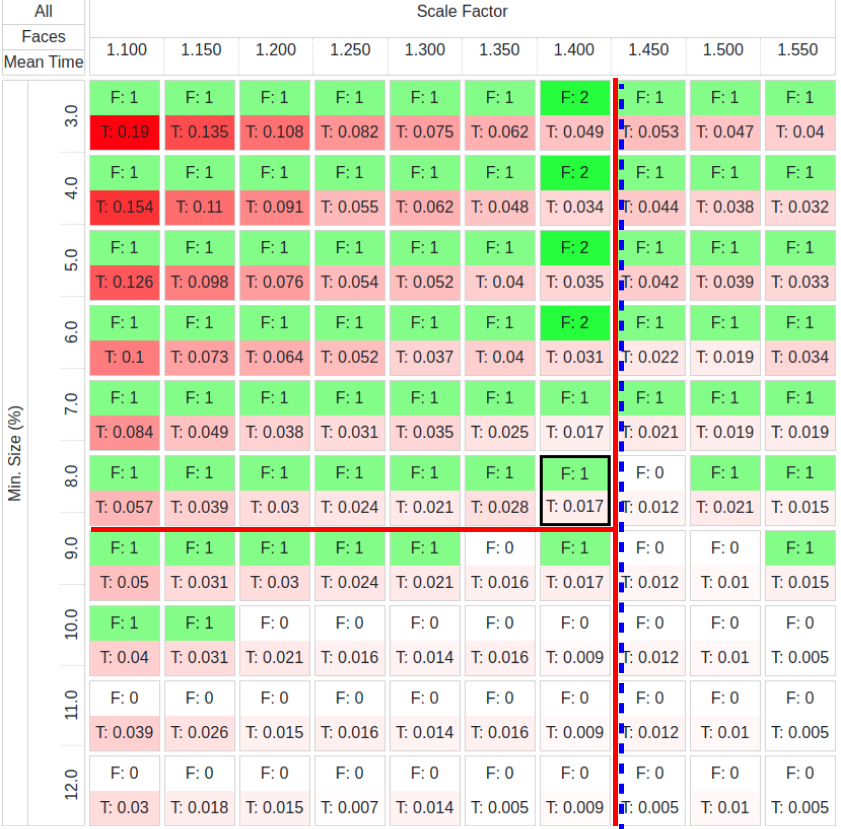
\includegraphics[width=0.49\textwidth]{Cap4_Experimentos_Realizados/Figures/cena2_800x600_pos2_matriz.jpg}
    \caption*{Fonte: autor.}
    \label{fig:otimizacaoCena2_600p_matrizes}
\end{figure}

\begin{figure}[H]
    \centering
    \caption[Otimização Cena 2 - resolução 600p - face detectada. À esquerda posição 1 e à direita, posição 2]{Otimização Cena 2 - resolução 600p - face detectada. À esquerda, posição 1, e à direita, posição 2.}
    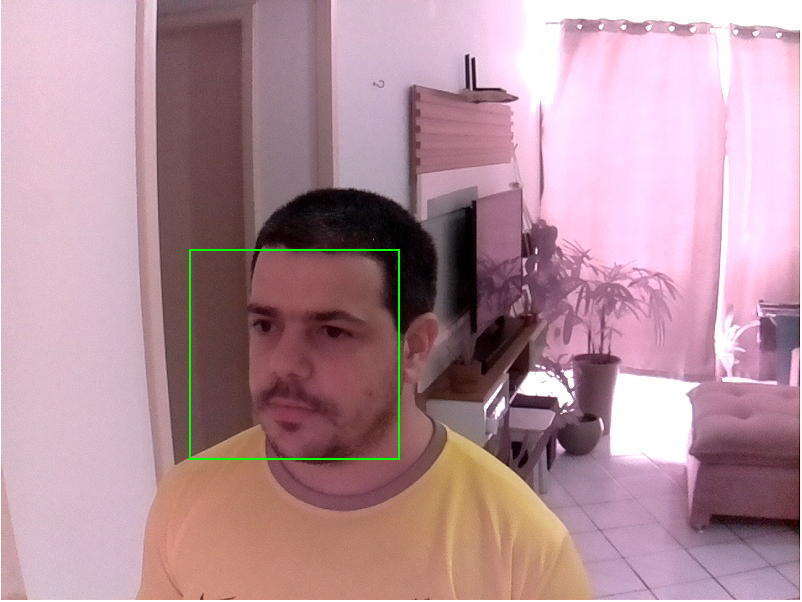
\includegraphics[width=0.49\textwidth]{Cap4_Experimentos_Realizados/Figures/cena2_800x600_pos1_face.jpg}
    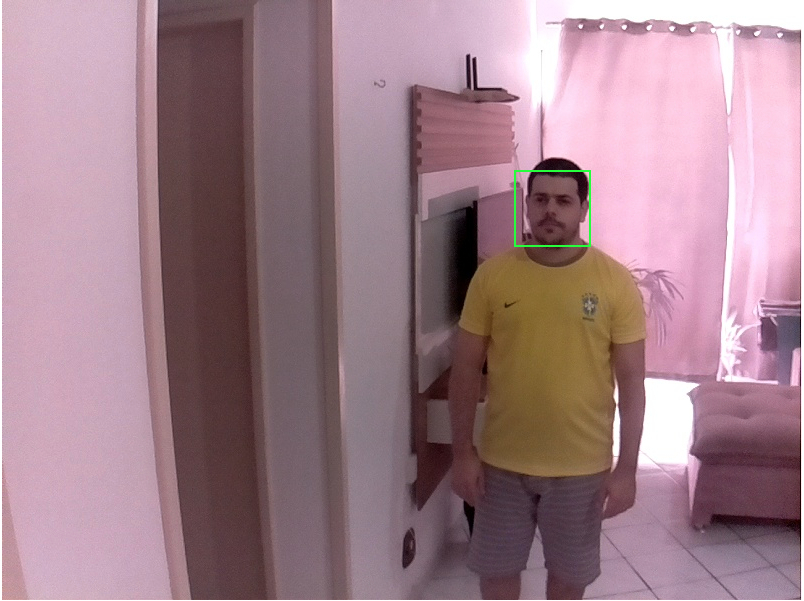
\includegraphics[width=0.49\textwidth]{Cap4_Experimentos_Realizados/Figures/cena2_800x600_pos2_face.jpg}
    \caption*{Fonte: autor.}
    \label{fig:otimizacaoCena2_600p_faces}
\end{figure}

\subsubsection{Resolução 480p} \label{sssec:resolution2-2}

\begin{figure}[H]
    \centering
    \caption[Otimização Cena 2 - resolução 480p - matrizes. À esquerda posição 1 e à direita, posição 2]{Otimização Cena 2 - resolução 480p - matrizes. À esquerda, posição 1, e à direita, posição 2.}
    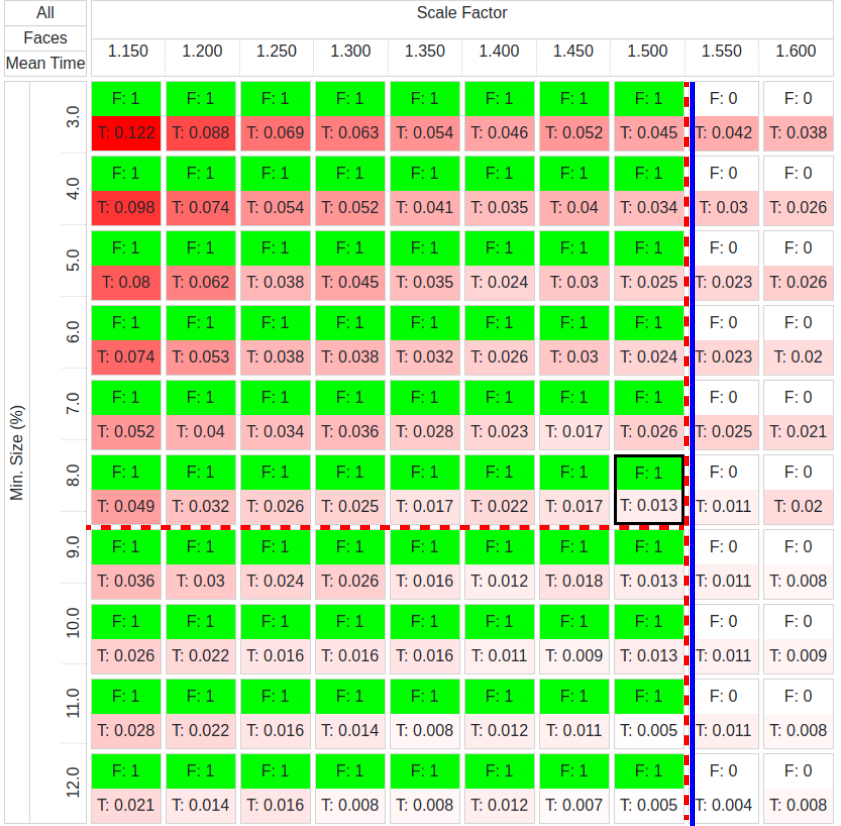
\includegraphics[width=0.49\textwidth]{Cap4_Experimentos_Realizados/Figures/cena2_640x480_pos1_matriz.jpg}
    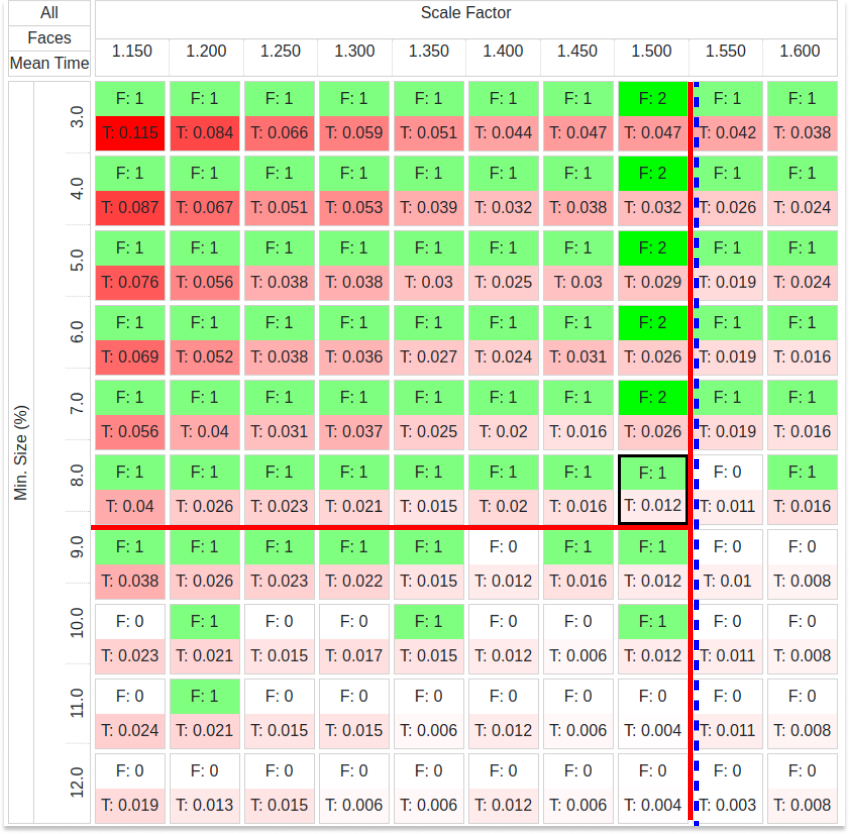
\includegraphics[width=0.49\textwidth]{Cap4_Experimentos_Realizados/Figures/cena2_640x480_pos2_matriz.jpg}
    \caption*{Fonte: autor.}
    \label{fig:otimizacaoCena2_480p_matrizes}
\end{figure}

\begin{figure}[H]
    \centering
    \caption[Otimização Cena 2 - resolução 480p - face detectada. À esquerda posição 1 e à direita, posição 2]{Otimização Cena 2 - resolução 480p - face detectada. À esquerda, posição 1, e à direita, posição 2.}
    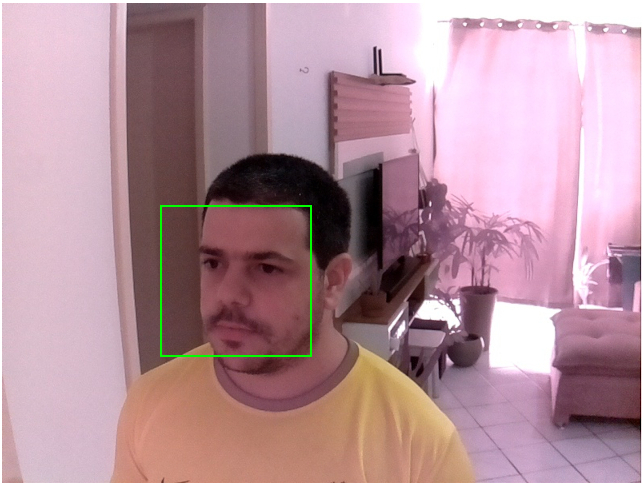
\includegraphics[width=0.49\textwidth]{Cap4_Experimentos_Realizados/Figures/cena2_640x480_pos1_face.jpg}
    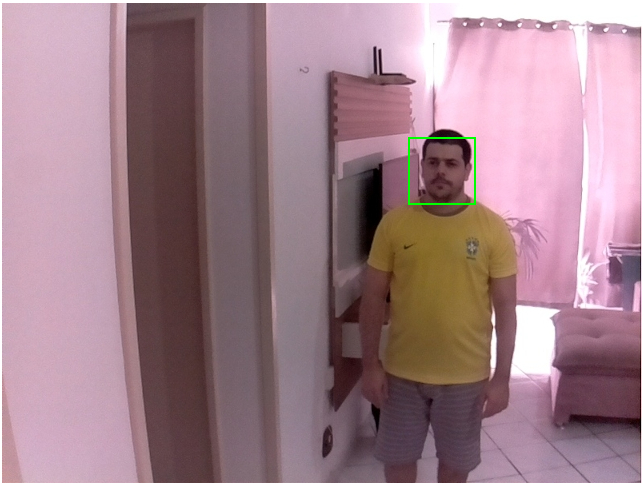
\includegraphics[width=0.49\textwidth]{Cap4_Experimentos_Realizados/Figures/cena2_640x480_pos2_face.jpg}
    \caption*{Fonte: autor.}
    \label{fig:otimizacaoCena2_480p_faces}
\end{figure}

\subsubsection{Resolução 240p} \label{sssec:resolution2-3}

\begin{figure}[H]
    \centering
    \caption[Otimização Cena 2 - resolução 240p - matrizes. À esquerda posição 1 e à direita, posição 2]{Otimização Cena 2 - resolução 240p - matrizes. À esquerda, posição 1, e à direita, posição 2.}
    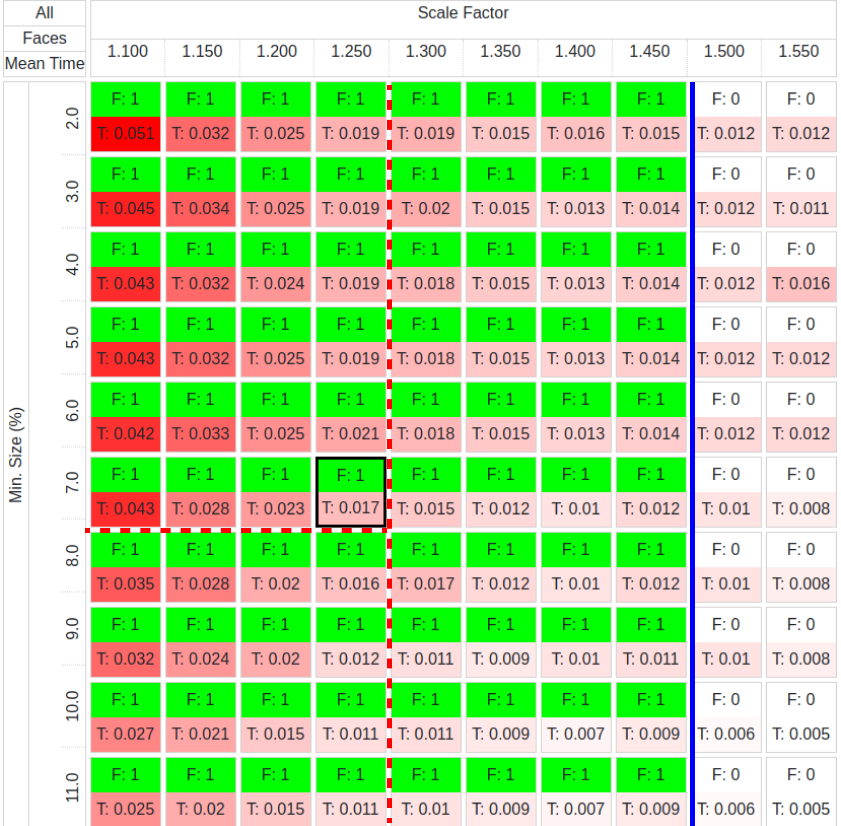
\includegraphics[width=0.49\textwidth]{Cap4_Experimentos_Realizados/Figures/cena2_320x240_pos1_matriz.jpg}
    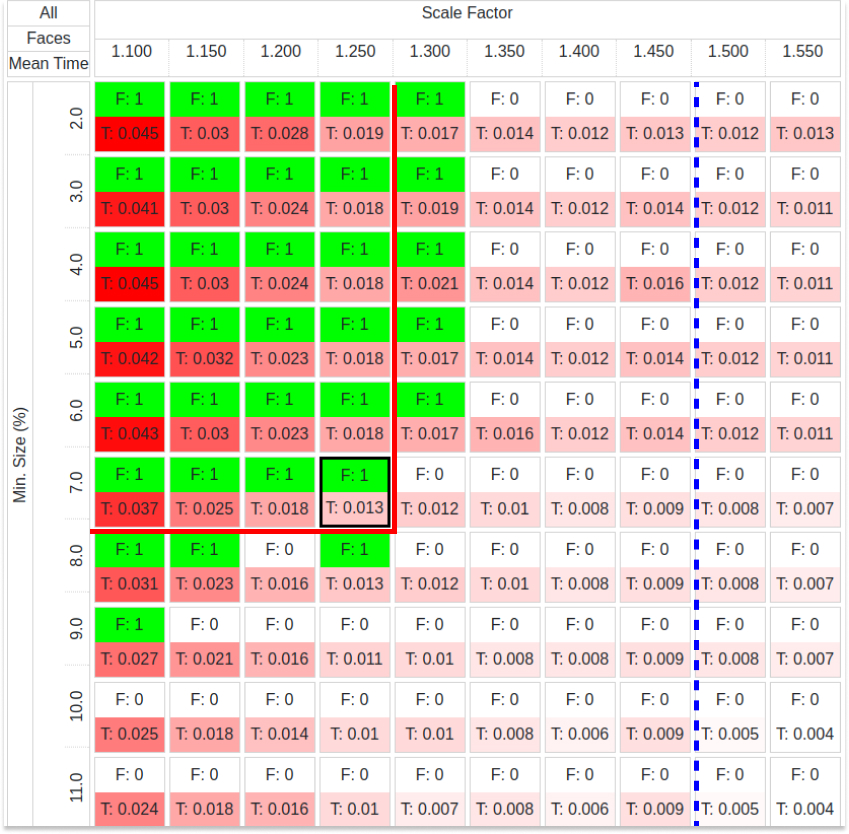
\includegraphics[width=0.49\textwidth]{Cap4_Experimentos_Realizados/Figures/cena2_320x240_pos2_matriz.jpg}
    \caption*{Fonte: autor.}
    \label{fig:otimizacaoCena2_240p_matrizes}
\end{figure}

\begin{figure}[H]
    \centering
    \caption[Otimização Cena 2 - resolução 240p - face detectada. À esquerda posição 1 e à direita, posição 2]{Otimização Cena 2 - resolução 240p - face detectada. À esquerda, posição 1, e à direita, posição 2.}
    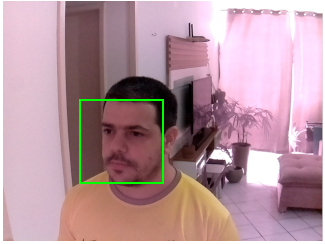
\includegraphics[width=0.49\textwidth]{Cap4_Experimentos_Realizados/Figures/cena2_320x240_pos1_face.jpg}
    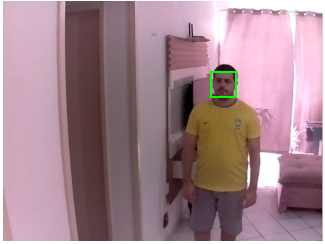
\includegraphics[width=0.49\textwidth]{Cap4_Experimentos_Realizados/Figures/cena2_320x240_pos2_face.jpg}
    \caption*{Fonte: autor.}
    \label{fig:otimizacaoCena2_240p_faces}
\end{figure}